%!TEX TS-program = xelatex
%!TEX encoding = UTF-8 Unicode

\documentclass[11pt]{article}
\usepackage[UKenglish]{babel}
\usepackage[UKenglish]{isodate} 
\usepackage[margin=2cm, a4paper]{geometry}
\usepackage{graphicx, fancyhdr}
\usepackage{fontspec, xltxtra, xunicode}
\usepackage{enumitem, tabu}

\setlist{noitemsep}

\usepackage{array, xcolor}
\definecolor{lightgray}{gray}{0.8}
\newcolumntype{L}{>{\raggedleft}p{0.16\textwidth}}
\newcolumntype{R}{p{0.8\textwidth}}
\newcommand\VRule{\color{lightgray}\vrule width 0.5pt}

\pagestyle{fancy}
\lhead{} % nothing
\chead{pbqk24}
\rhead{} % nothing
\lfoot{} % nothing
\cfoot{\thepage}
\rfoot{} % nothing

\title{\vspace{-6.0ex}Structure from Motion: creating a 3D world from an image sequence\\\vspace{1.0ex}\large Advanced Computer Vision Assignment}
\author{pbqk24}
\date{6 December 2018}

\begin{document}
	\maketitle
	
\section*{Approach to the Problem}
The solution implements the general Structure from Motion pipeline, specifically for 3D terrain point cloud creation, composed of the general steps below for each image pair:
\begin{enumerate}
	\item Feature point extraction
	\item Feature point matching between the images
	\item Estimation of the Fundamental matrix through RANSAC on the feature matches
	\item Computation of the Essential matrix
	\item Computation of relative camera matrix (rotation and translation) of the second camera from the first
	\item Camera matrix composition to produce global camera matrix of the first and second camera
	\item Triangulation of matched feature points to produce 3D points
	\item Creation and plotting of 3D point cloud for visualization
\end{enumerate}

At each part of the pipeline, filtering was performed and the parameters used were tuned in order to improve the output. Firstly, SURF features were extracted from the images with a hessian threshold of 750. Compared to using a lower threshold, this yielded nearly identical results while being significantly faster. For the feature point matching, a brute force matcher was used to ensure the best matches were found, and a ratio test was performed with a ratio of 0.7 to filter out non-unique matches. This improved the set of matches and minimised the number of obviously false matches produced. An example of this is shown in figure \ref{fig:featurePointMatches}.

\begin{figure}[h]
	\centering
	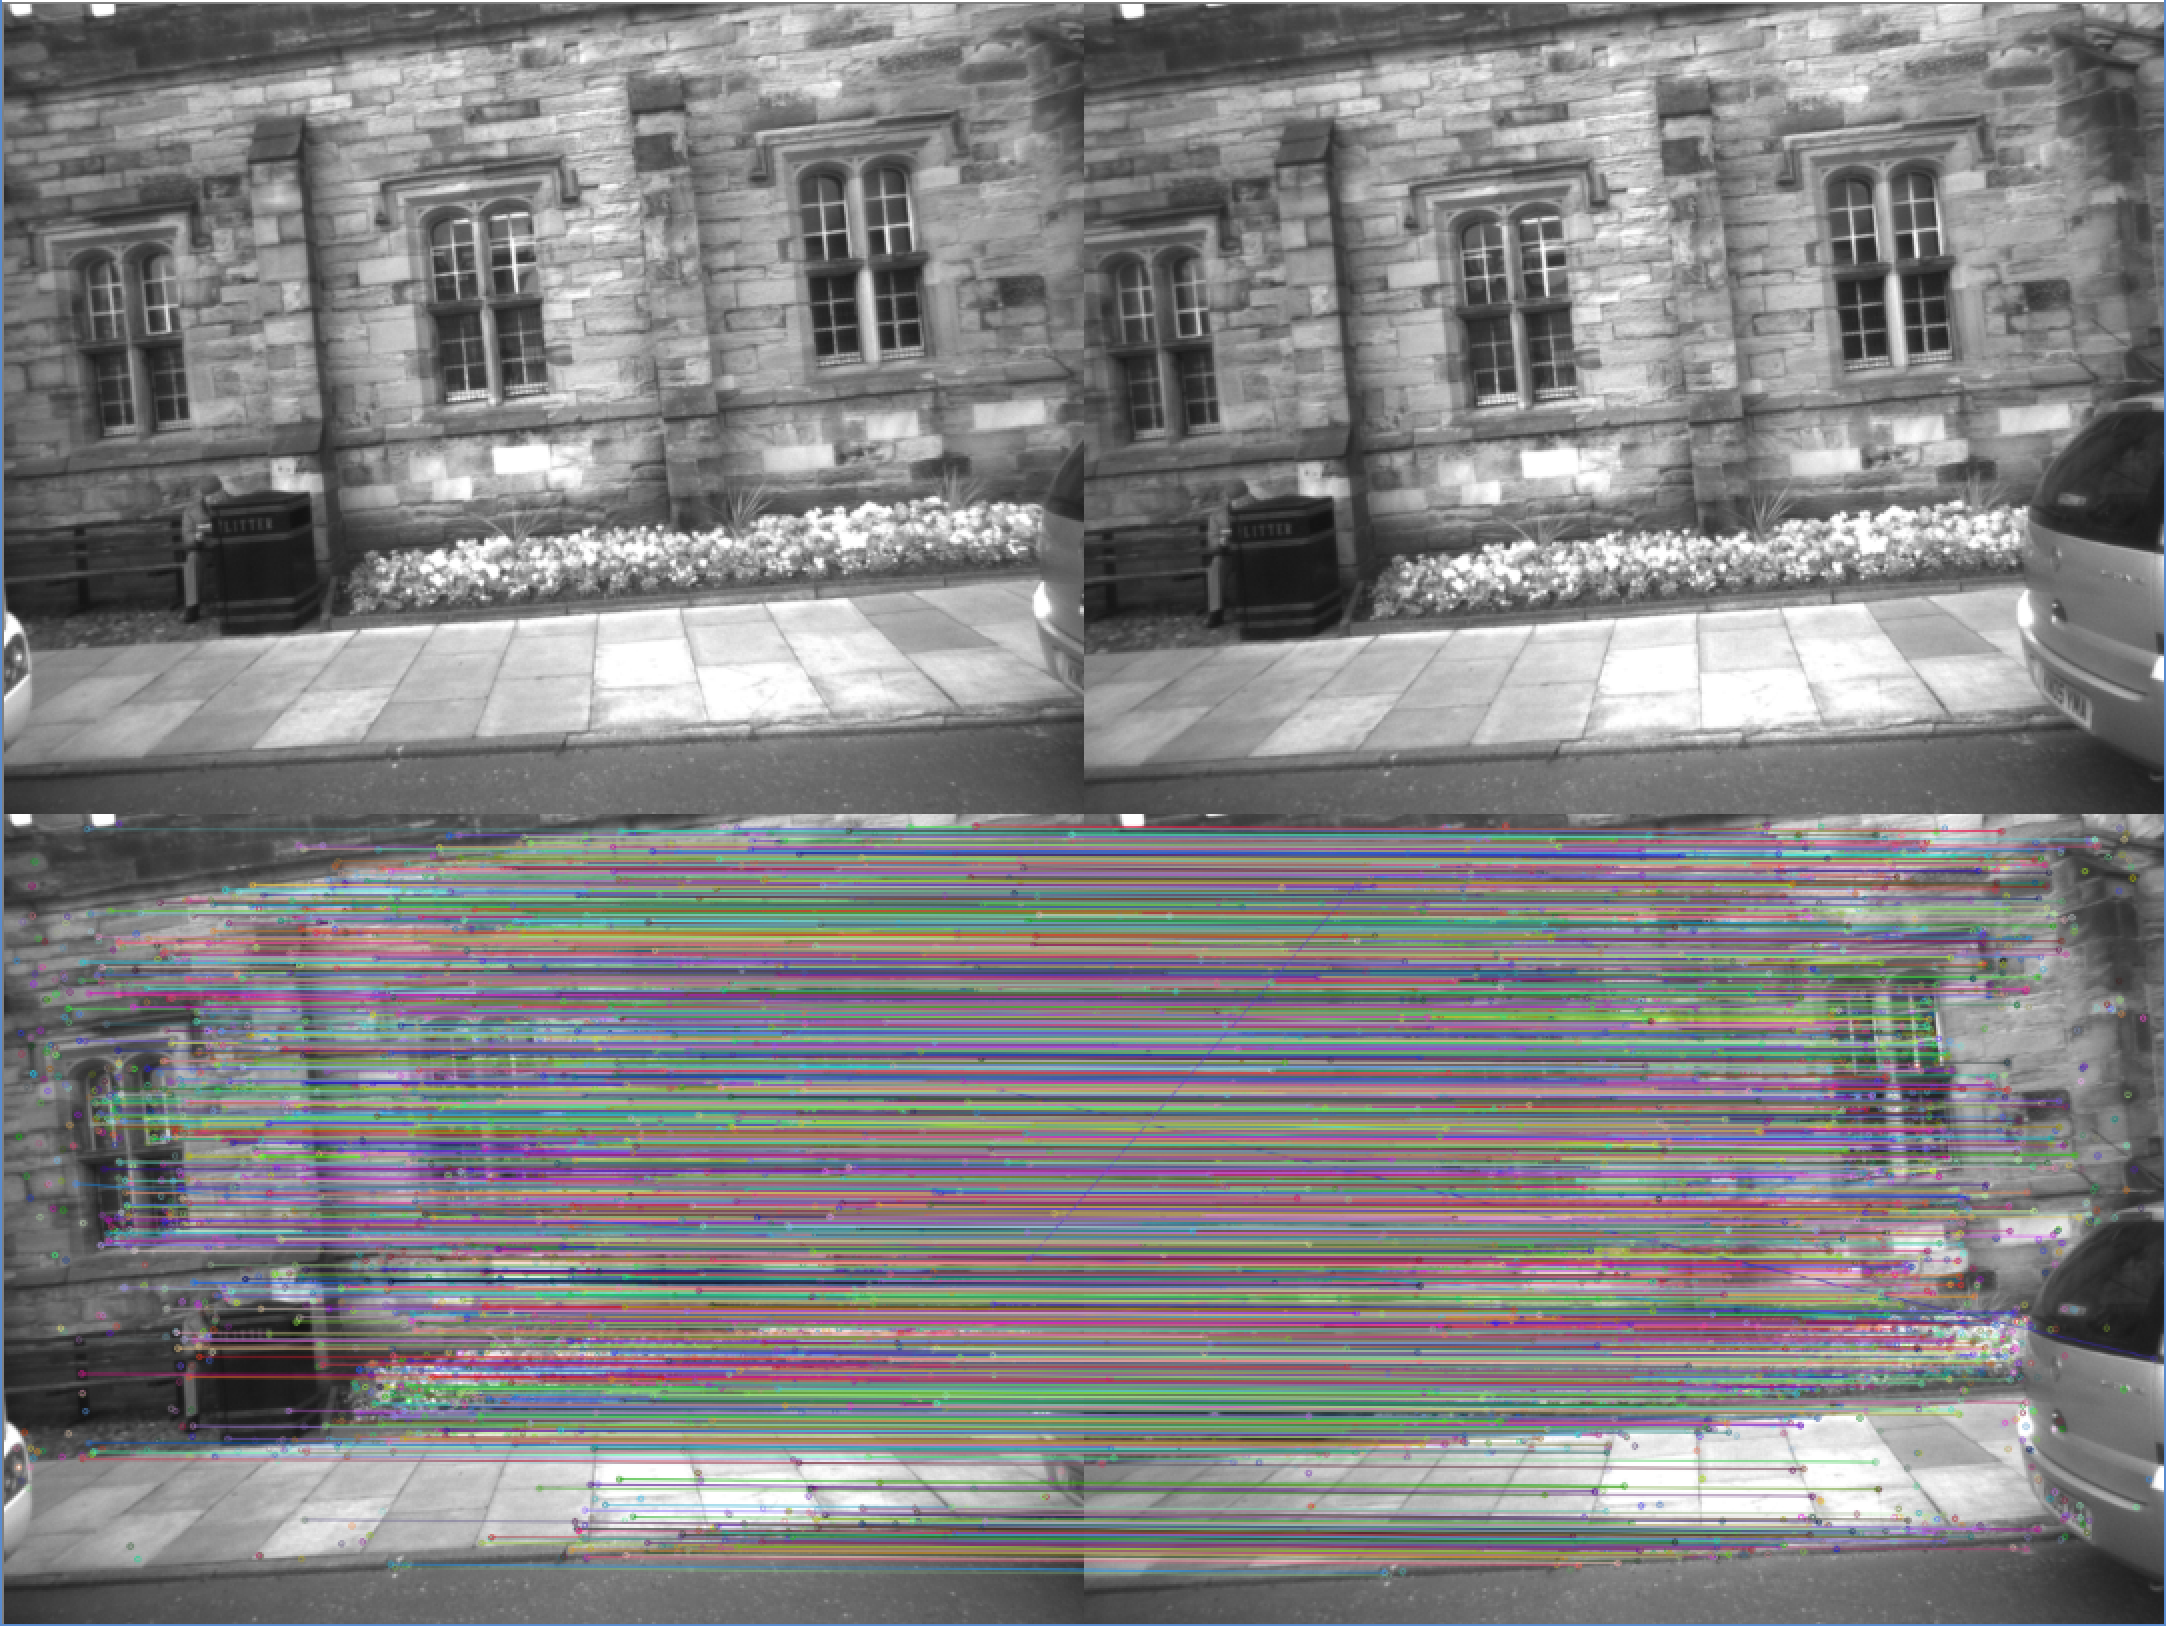
\includegraphics[scale=0.42]{featurePointMatches}
	\caption{Remaining feature point matches between the first two images of sequence 2 left after filtering. Nearly all matches have the same angle, with only a couple noticeable outliers. The top half plots the input images, while the bottom plots the extracted feature points and matches.}
	\label{fig:featurePointMatches}
\end{figure}

In step 3, estimating the Fundamental matrix (F), a distance threshold of 0.3 and a confidence level of 0.999 was used. These parameters ensured that a good F was found: if a higher distance threshold was used the F would be too inaccurate for the rest of the processing, and a lower distance threshold meant very few of the point matches were inliers with F. Only the inliers with F were passed further through the pipeline, ensuring only those points that were accurately mapped between the images influenced the output.

After computing the Essential matrix (E), these inliers were used to compute the geometric relationship [R|t] between the two cameras. As part of this, the inliers were further filtered to only include points which, when plotted in 3D, were in front of both of the cameras. At this point, the resulting [R|t] matrix and the inlier points were checked to ensure good results. This was done through requiring a z translation value in the range $[-0.05, 0.05]$ and at least 50 inliers. This was based on the cameras being mounted on a car, which cannot (normally) translate sideways (in the z axes of the cameras). Also, if the [R|t] matrix resulted in very few inliers the point cloud was likely inaccurate, so a requirement was placed on this. If the output did not meet these requirements the process was repeated from estimating F up to 30 times. After this, the image was skipped. This process drastically improved the quality and coherence of the final point cloud.

Finally, the [R|t] matrix was composed with the global [R|t] of the previous camera to produce the next camera's global [R|t], and both of these were used to triangulate the remaining inliers, which were then plotted.

\section*{Performance Achieved}
The pipeline achieves very good results on four of the six sequences in the sample data. In these sequences, shown in figures \ref{fig:2_left_gray} to \ref{fig:4_left_depth}, the point clouds generally adhere to the scene in question, although with a fair amount of outliers. In each the general structure of the scene is captured, and main components, such as the wall of buildings in sequence 2 left, are noticeably present.

\begin{figure}[h]
	\centering
	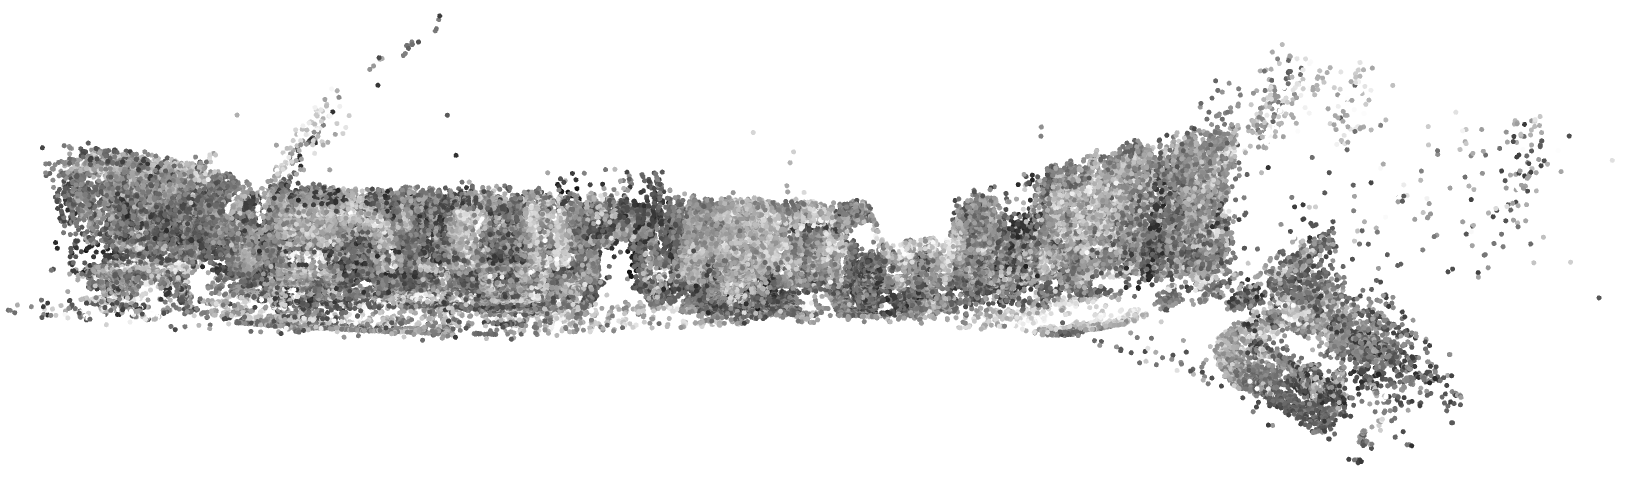
\includegraphics[scale=0.65]{Sequence2Left_Grayscale}
	\caption{Sequence 2 Left, Grayscale colour extracted from the 2D points in the input images. The cloud plots the wall of buildings between the cathedral and the castle, and the entrance to the castle (right side).}
	\label{fig:2_left_gray}
\end{figure}
\begin{figure}[h]
	\centering
	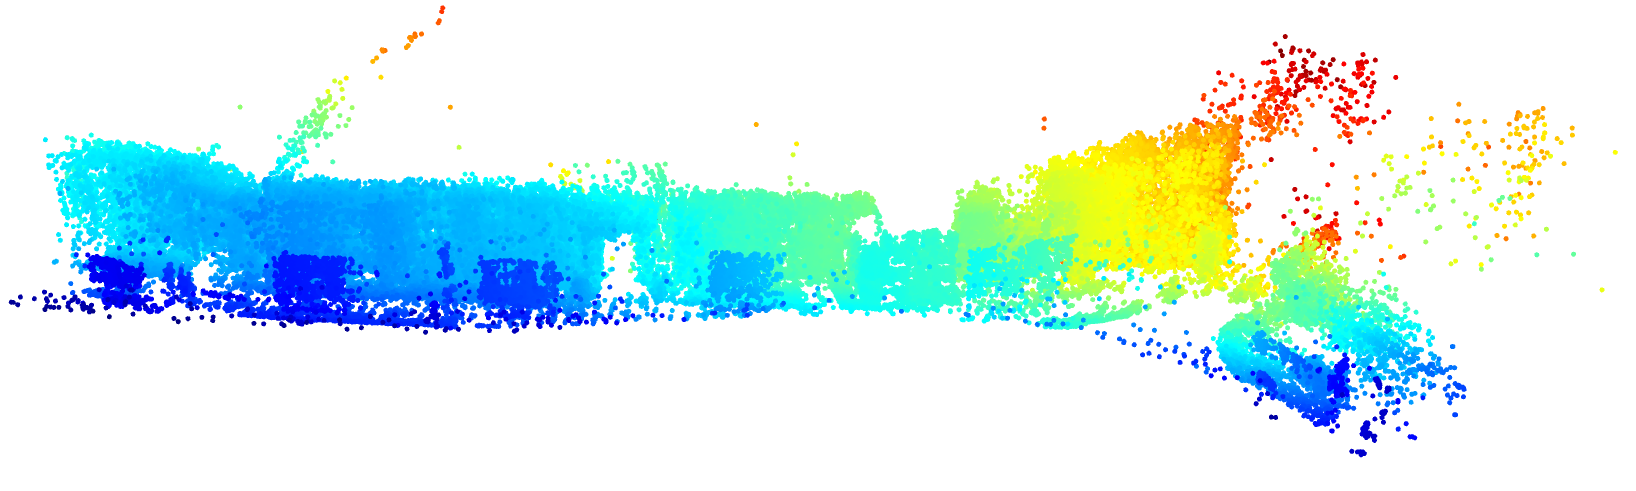
\includegraphics[scale=0.65]{Sequence2Left_Depth}
	\caption{Sequence 2 Left, Colour corresponding to Depth from camera. Note the individual point clouds, usually in dark blue, that jump out from the wall, caused by missing frames in the dataset.}
	\label{fig:2_left_depth}
\end{figure}

Some shortcomings in the results include sets of point clouds that appear much closer to the camera positions than expected, mentioned in figure \ref{fig:2_left_depth} and figure \ref{fig:3_left_depth}. These are caused by missing frames in the dataset, where the distance moved by the car/camera between two consecutive images is drastically increased, which results in much lower depth (z-axis) values of the point cloud due to the lack of absolute scale in the plots. Additionally, as no bundle adjustment is performed smaller structures are hard to pick out as the positions of a given point varies a lot between image pairs.

\begin{figure}[h]
	\centering
	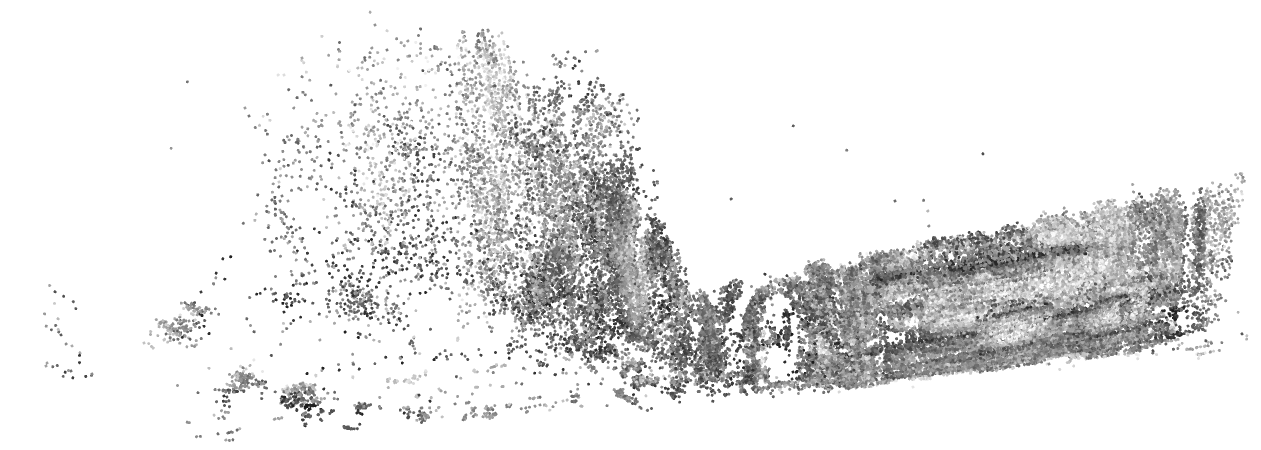
\includegraphics[scale=0.7]{Sequence3Left_Grayscale}
	\caption{Sequence 3 Left, Grayscale colour from 2D images. The left side corresponds to market square, the right side shows the front of the church at the bottom of the square}
	\label{fig:3_left_gray}
\end{figure}
\begin{figure}[h]
	\centering
	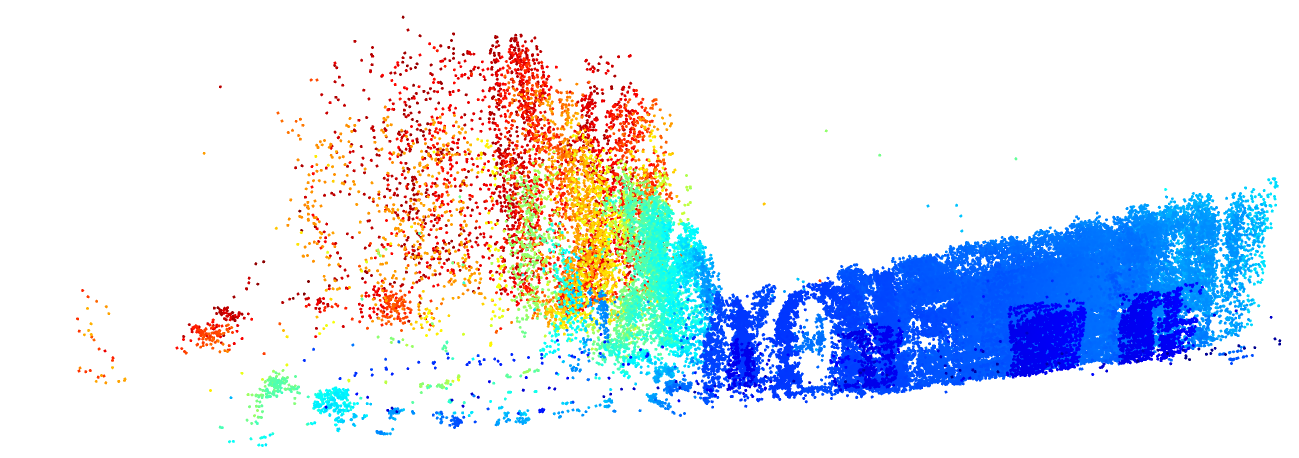
\includegraphics[scale=0.7]{Sequence3Left_Depth}
	\caption{Sequence 3 Left, Colour corresponding to Depth from camera. Note again the presence of individual point clouds (in dark blue, on the right) appearing closer than expected.}
	\label{fig:3_left_depth}
\end{figure}

The poor sequences, sequence 2 right (figures \ref{fig:2_right_gray} and \ref{fig:2_right_depth}) and sequence 4 right (figures \ref{fig:4_right_gray} and \ref{fig:4_right_depth}), likely had problems due to the large distance of most objects from the camera. Due to this, very few feature points were found in each image, and the quality of the point matches also suffered. Additionally, due to the distance, any error in F or [R|t] had a much larger impact than in the other sequences.

\begin{figure}[h]
	\centering
	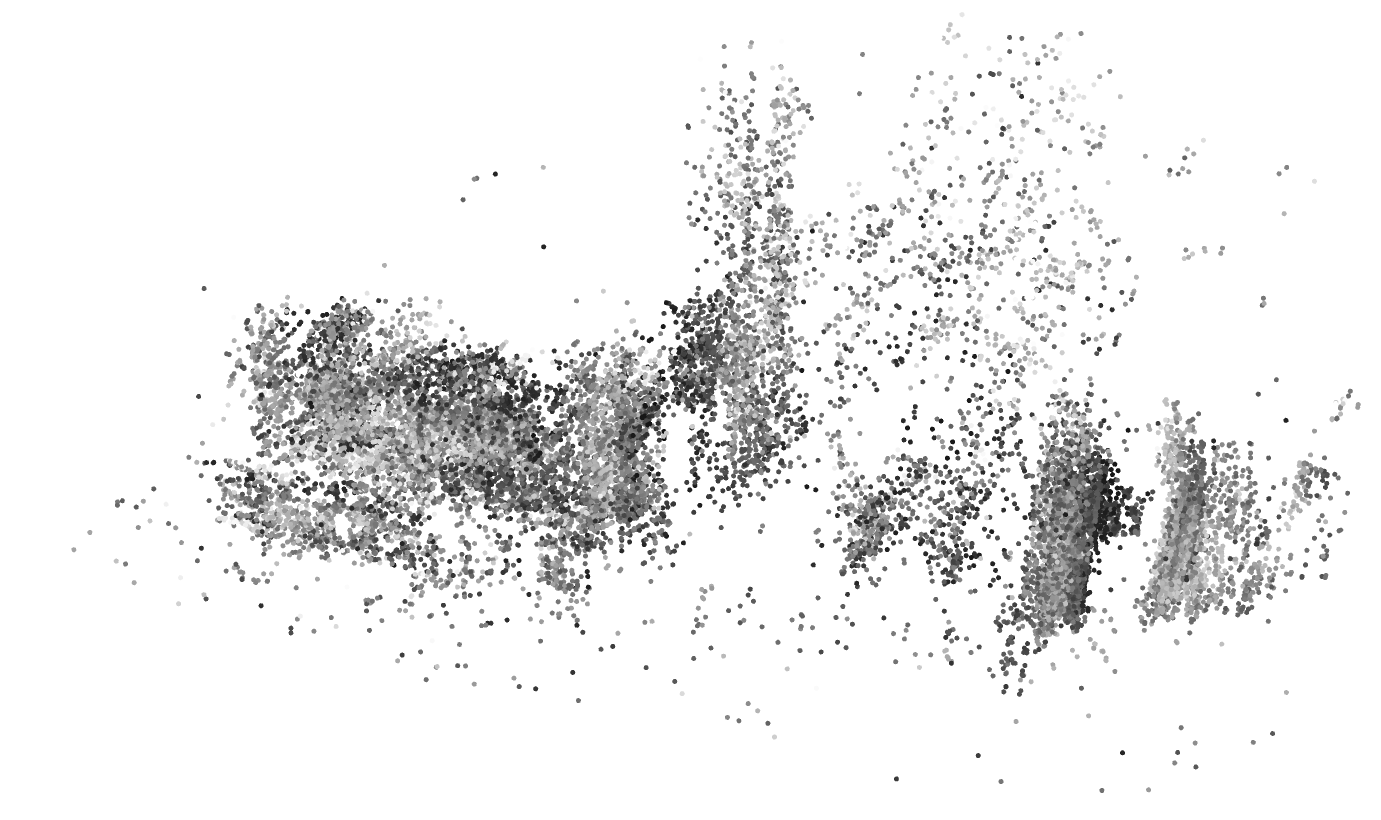
\includegraphics[scale=0.5]{Sequence3Right_Grayscale}
	\caption{Sequence 3 Right, Grayscale colour from 2D images. The cloud plots a side road on Market Square next to Boots. Note the doors on either side of the road, in the center of the cloud.}
	\label{fig:3_right_gray}
\end{figure}
\begin{figure}[h]
	\centering
	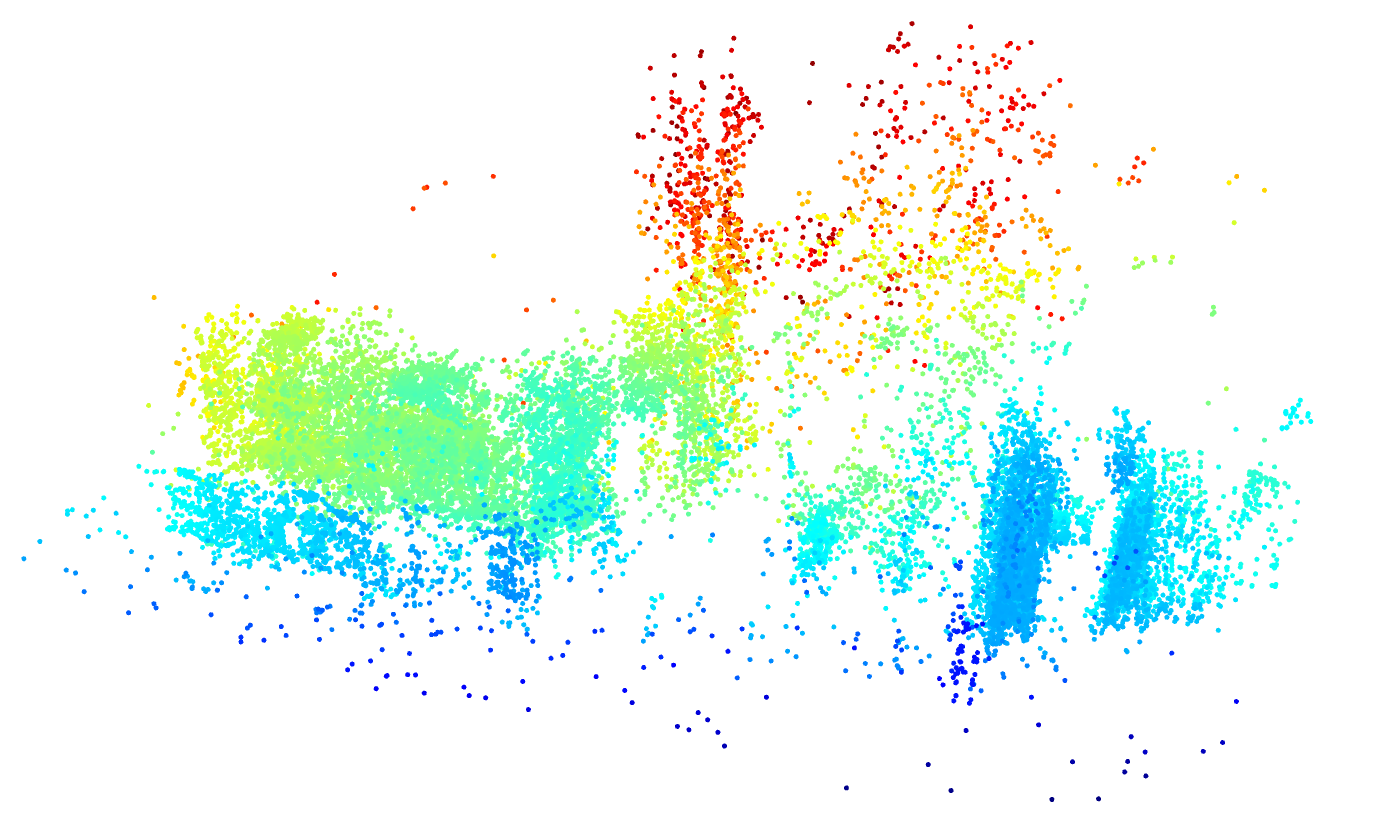
\includegraphics[scale=0.5]{Sequence3Right_Depth}
	\caption{Sequence 3 Right, Colour corresponding to Depth from camera. Note the number of points plotted on the road leading away from the camera (red/warmer coloured section).}
	\label{fig:3_right_depth}
\end{figure}

\begin{figure}[h]
	\centering
	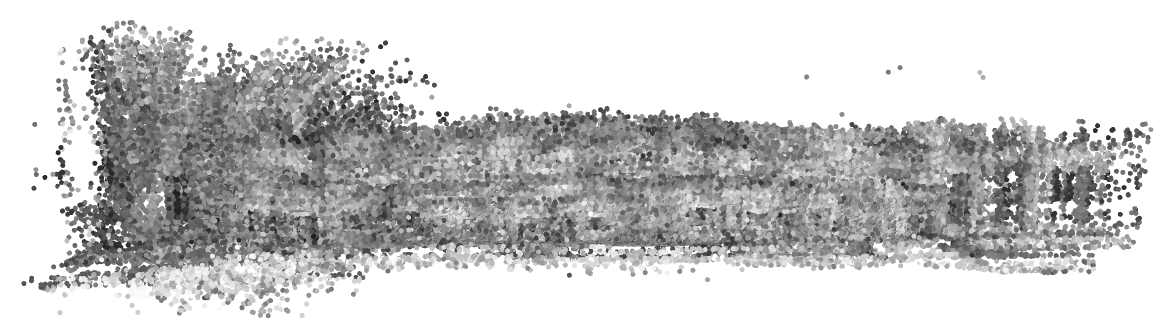
\includegraphics[scale=0.6]{Sequence4Left_Grayscale}
	\caption{Sequence 4 Left, Grayscale colour from 2D images, plotting a section of houses on Palace Green. Note the consistency of the point cloud in the right section.}
	\label{fig:4_left_gray}
\end{figure}
\begin{figure}[h]
	\centering
	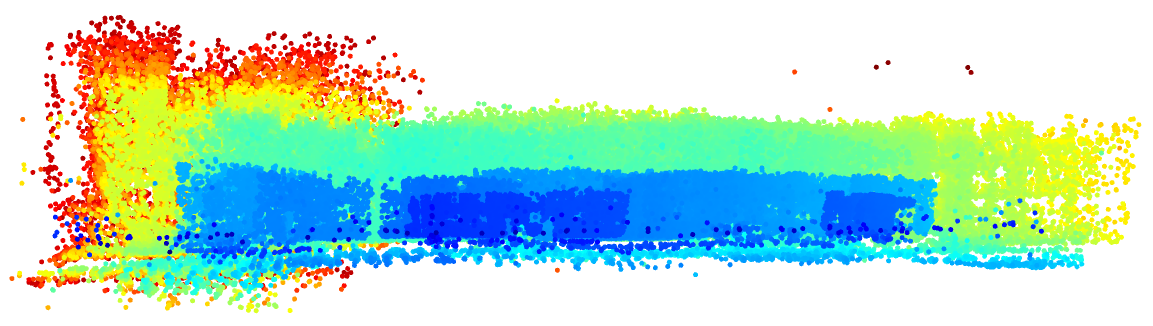
\includegraphics[scale=0.8]{Sequence4Left_Depth}
	\caption{Sequence 4 Left, Colour corresponding to Depth from camera. As in figures \ref{fig:2_left_depth} and \ref{fig:3_left_depth} there are a few point clouds that jump out of the wall (dark blue).}
	\label{fig:4_left_depth}
\end{figure}

\begin{figure}[h]
	\centering
	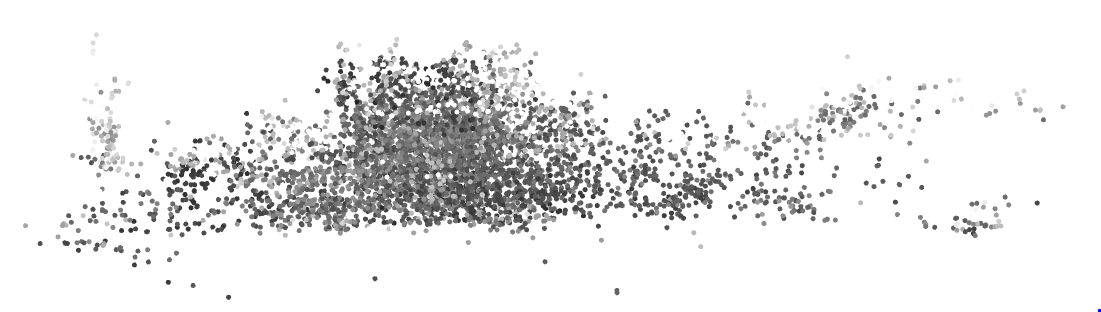
\includegraphics[scale=0.8]{Sequence2Right_Grayscale}
	\caption{Sequence 2 Right, Grayscale colour from 2D images. The cloud is quite sparse, but the general shape of a building can be seen in the left part of the cloud.}
	\label{fig:2_right_gray}
\end{figure}
\begin{figure}[h]
	\centering
	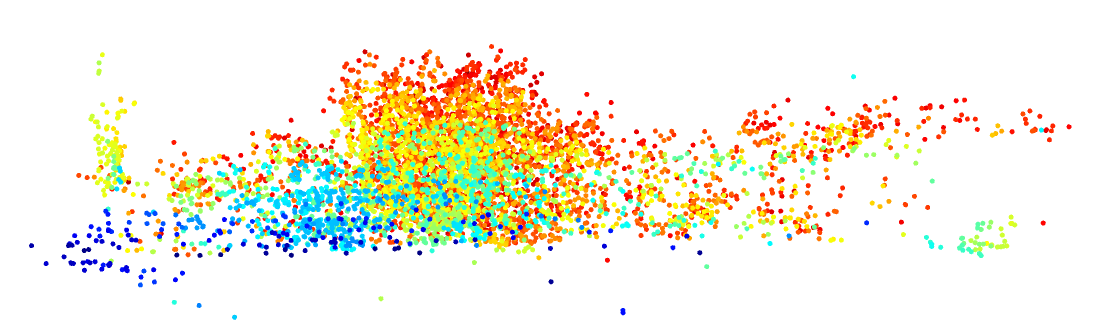
\includegraphics[scale=0.8]{Sequence2Right_Depth}
	\caption{Sequence 2 Right, Colour corresponding to Depth from camera. The mix of colours in the area of the building show the varying depths calculated for different image pairs, resulting in inconsistent output.}
	\label{fig:2_right_depth}
\end{figure}

\begin{figure}[h]
	\centering
	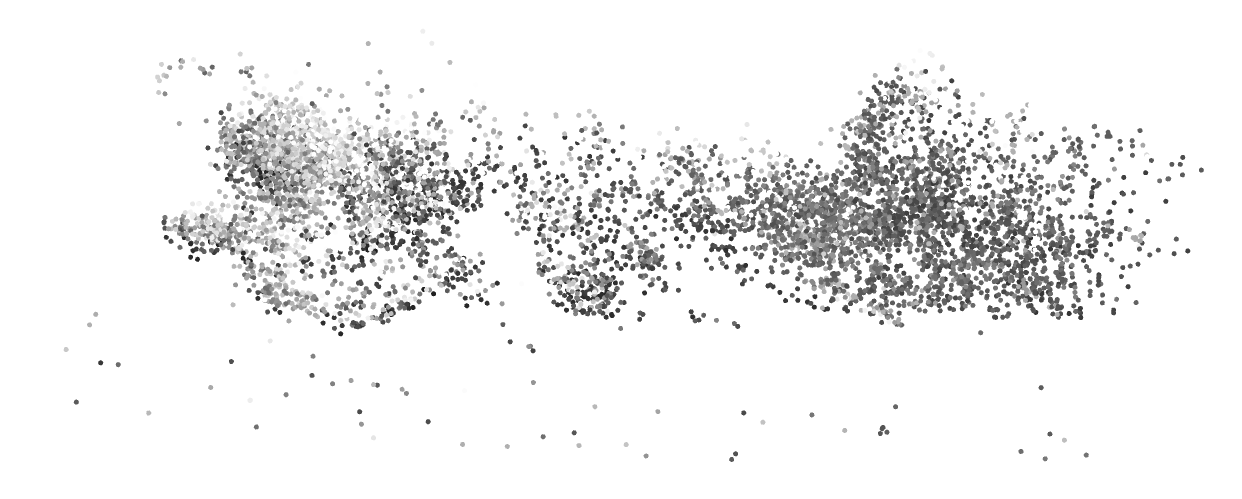
\includegraphics[scale=0.8]{Sequence4Right_Grayscale}
	\caption{Sequence 4 Right, Grayscale colour from 2D images. Again, the general shape of a building can be noticed on the right, though overall the point cloud is very inconsistent.}
	\label{fig:4_right_gray}
\end{figure}
\begin{figure}[h]
	\centering
	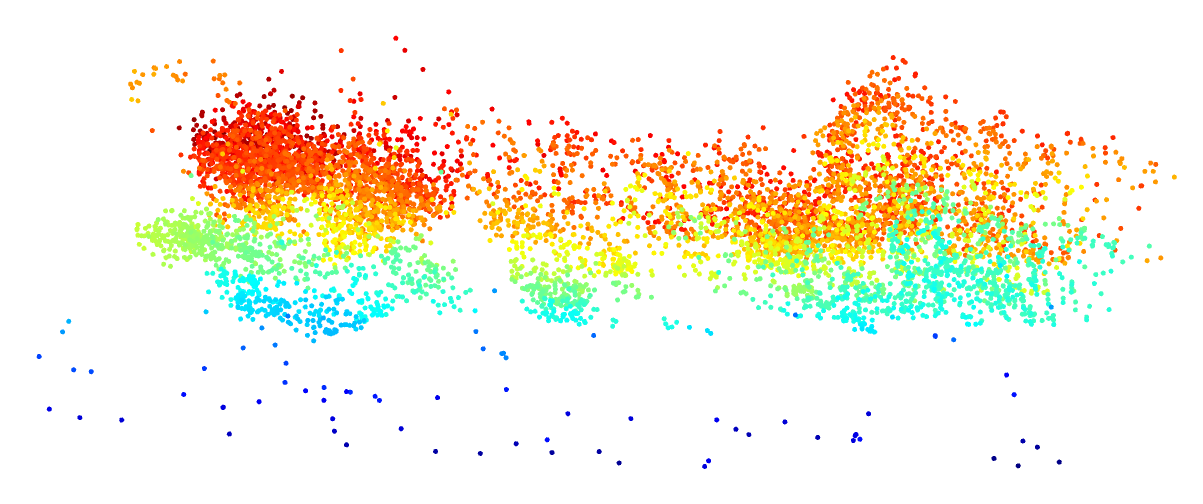
\includegraphics[scale=0.8]{Sequence4Right_Depth}
	\caption{Sequence 4 Right, Colour corresponding to Depth from camera. Similar problems are noticed as in figure \ref{fig:2_right_depth}, though to a lesser extent.}
	\label{fig:4_right_depth}
\end{figure}


\end{document}